\newpage
\fancyhead[C]{Thomas Turner}
\section{Intra-UAV Communication Architecture} \label{Intra Communication}

\subsection{Introduction}\label{sub_section:tgt_intra_com_intro}
The communication and networking of devices on our device is a key consideration for design. All interfaces and software should be as uniform as possible as they reduce integration complexity of creating new components for specific environments, applications, regulations and general upgrades.

\subsection{Design Considerations}\label{sub_sub_section:tgt_intra_comms_design_considerations}

\subsubsection{Modularity}\label{sub_sub_section:tgt_modularity}
\paragraph{Relevance}
Mechanical modularity is the most obvious path as the components need to physically connect easily. However, the communication architecture also needs to support this so that devices can easily communicate even if they are changed completely.
\paragraph{Modular Communication Protocols}
Defined interfaces, protocols and pin allow for different devices to communicate without specific dependencies on each other. Therefore, integrating new sensors or modules does not require a new communication system. Another key property of modular networks is physical, some networks lend themselves better to modular design, for example for a \gls{CAN} FD Bus you only need to add a stub and all interfaces should use standard connectors.

\subsubsection{Telemetry}\label{sub_sub_section:tgt_telemetry}
\paragraph{Battery Telemetry}
The two key failure modes for the battery are state of charge and thermal runaway. Both can cause complete failure and therefore both should be monitored during flight. This allows for \gls{RTH} to be triggered in case of a state of charge or emergency landing in the case of thermal runaway. Therefore, real-time telemetry is sent from the \gls{BMS} to the flight controller for temperature and state of charge.
\paragraph{\gls{ESC} Telemetry}
Providing \gls{ESC} telemetry for voltage, current and \gls{RPM} is important information when classifying motor and propeller faults accurately which is needed to support the adaptive control strategy in Section \ref{sub_sub_section:tgt_actuator_fault}. Furthermore, \gls{ESC} temperature is also sent to monitor for overheating. 

\subsubsection{Communication Bus}\label{sub_sub_section:tgt_bus}
\paragraph{\gls{CAN} bus}
In order to support the \gls{ESC} telemetry required Cyphal should be used as it is widely supported by \gls{COTS} hardware and can run over \gls{CAN} bus. CAN Flexible Data (FD) is widely used and supported and can process data transfer speeds up to 8 Mbps using the transceiver used in Section \ref{section:Custom Hardware}\footnote{\url{https://www.ti.com/lit/ds/symlink/tcan1472-q1.pdf}} whilst also supporting modularity. In order to guarantee redundancy a dual \gls{CAN} bus is selected so if there is a failure on one bus, the other bus is used. Failures can be detected across the bus as all modules will communicate 10 Hz heartbeats to each other indicating that they are operating as normal so if this heartbeat is not received the redundant bus is used instead. This allows for failure handovers in just 0.1s. Lastly, as \gls{CAN} is a differential signal the lines are carried in a twisted pair and transferred in a sheaf to reduce \gls{EMI} and risk of damage. 
\paragraph{Imaging Separation}
The images used in GPR and Thermal require significantly more data then both telemetry and command signals. Therefore, they are separately connected to the on-board computer using 1000BASE-T Gigabit Ethernet supporting data transfer speeds up to 1 Gbps. It also utilises a copper twisted pair and differential signal for noise rejection \cite{Ethernet}.  This supports thermal and GPR imaging in addition to future upgrades and increased data transfer rates.
\paragraph{Node Distribution}
Safety critical devices ensure that the drone does not sustain damage or isolate itself. This includes components necessary for flight and the sensors required for \gls{RTS} explored in Section \ref{Return to Safety}. To ensure that failures are minimised, safety critical devices should be redundant. If a safety critical device does not have a redundant version it should be able to communicate on at least two different lines preventing a single module failure causing device failure. Distributing the devices on different communication lines reduces the risk of failure as it reduces the risk of common mode failure. For example, if a \gls{GNSS} module were to have an improper fixture and move in a way that it severs all connections; if both communication lines are in it, both are severed. However, if it is on only one communication line then the other communication line is undamaged. This layout is shown in Figure \ref{fig:CAN_bus}. 
 \begin{figure}[h]
 \centering
  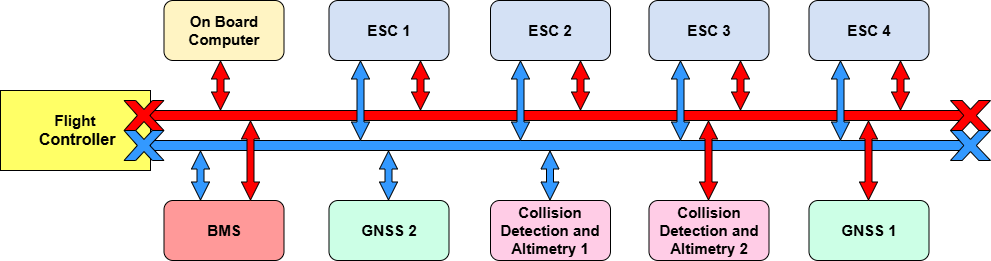
\includegraphics[width=1\textwidth]{figs/Thomas/Intra Communication/CAN bus.png}
 \caption{Bus layout}
 \label{fig:CAN_bus}
 \end{figure}
\paragraph{Communication Architecture}
Centralised architectures consist of a central node directly connected to all the relevant devices. while this is a simple and cost effective method it leaves the device to single points of failure. In order to build robustness, the custom \gls{GNSS} module is capable of independently executing landing and \gls{RTS} as it is equipped with an independent \gls{IMU} that is control capable. The \gls{GNSS} module sends control signals if the flight controller is no longer received ensuring smooth handover. 
\paragraph{High Level Protocol}
A single high level protocol being used across all components makes the \gls{UAV} more adaptable and makes hiring developers easier. This is because a single skill-set can interact with the entire system. Therefore, Cyphal will be used as it can operate over \gls{CAN} and Ethernet which are the key communication systems. It is used over alternative application protocols including ROS 2 and Mavlink as it has wider support from \gls{COTS} \gls{ESC}s\footnote{\url{https://opencyphal.org/}} . 

\subsection{Conclusion}
All major communication interfaces are considered and allocated suitable protocols. The dual \gls{CAN} design supports modularity and redundancy, the Ethernet connection between imaging sensors and the onboard computer supports the high data transfer rates required and future upgrades. Lastly, by using Cyphal as a common high level application protocol the system is easier to learn and use whilst also being supported widely by \gls{COTS} hardware.